% ==============================================================================
% CHAPTER 1: THE ROLE OF STATISTICS IN ENGINEERING
% ==============================================================================

\section*{The Role of Statistics in Engineering}

To illustrate the fundamental importance of probability and statistics in engineering,
we start by looking at two practical examples drawn from the bachelor \textbf{Military Systems and Technology}.

\begin{example}[Maintenance: reliability of a circuit]

    Consider a network circuit that functions only if there exists an unbroken path of operational components leading from the left terminal to the right terminal. 
    The system depicted in \Cref{fig:example_circuit} consists of three distinct components.
    Devices $A$ and $B$ are connected in parallel, and Device $C$ is connected in series with the parallel pair.\medskip

    \begin{center}
        \begin{tikzpicture}[>=stealth]
            \def\shift{2/3}
            \foreach \label/\x/\y in {A/0/1, B/0/-1, C/2/0}
            {
                \node[device] (device\label) at (\x, \y) {$\label$};
            }

            \coordinate (topleft) at ($(deviceA.west)+(-\shift,0)$);
            \coordinate (topright) at ($(deviceA.east)+(\shift,0)$);
            \coordinate (bottomleft) at ($(deviceB.west)+(-\shift,0)$);
            \coordinate (bottomright) at ($(deviceB.east)+(\shift,0)$);

            \coordinate (leftAB) at ($(topleft)!.5!(bottomleft)$);
            \coordinate (rightAB) at ($(topright)!.5!(bottomright)$);

            \draw (deviceA) -- (topleft) -- (bottomleft) -- (deviceB);
            \draw (deviceA) -- (topright) -- (bottomright) -- (deviceB);

            \draw (leftAB) -- ++(-2*\shift,0);
            \draw (rightAB) -- (deviceC);
            \draw (deviceC) -- ++(2*\shift,0);

        \end{tikzpicture}
        \captionof{figure}{Circuit configuration with three operational devices.}
        \label{fig:example_circuit}
    \end{center}\medskip

    Due to the system geometry, the circuit successfully operates if Device $C$ and at least one of Devices $A$ or $B$ function properly. 
    Conversely, if Device $C$ fails, the entire circuit fails regardless of the states of $A$ and $B$.\medskip

    Suppose now that each individual device has an expected average lifetime of $10$ hours.
    We wish to answer the following question: \textbf{what is the probability that the overall circuit remains operational for at least 9 hours?} \medskip

    We analyze this scenario under two different modeling perspectives:\medskip

    \begin{itemize}\setlength\itemsep{1em}
        \item From a \textbf{deterministic perspective}, variability is completely ignored.
        In other words, all devices are assumed to operate for exactly their expected lifetime of $10$ hours.
        Under this assumption, every component is guaranteed to survive past $9$ hours. 
        Consequently, the probability that the system operates for at least $9$ hours is equal to $1$ (or \SI{100}{\percent}).

        \item From a \textbf{stochastic perspective}, we take into account that component lifespans exhibit random fluctuations and variability.
        When incorporating random variation (modeling lifespans as random variables), the actual probability drops significantly to approximately $0.52$ (or \SI{52}{\percent}).\medskip

        This result can be verified through Monte Carlo simulation (using software such as Excel) or calculated analytical methods in probability theory.
        In a simulation approach, we simulate $10{.}000$ independent trials of the circuit (see \enquote{Excel Simulation - Learning Task 1}):
        
        \begin{enumerate}\setlength\itemsep{1em}
            \item For each trial, three individual lifespans are pseudo-randomly generated for $A$, $B$, and $C$ according to an appropriate failure distribution.
            \item The total lifespan of the system is computed in Column $D$ as $\min(\max(A, B), C)$.
            \item Column $E$ evaluates whether the overall circuit lifespan exceeds $9$ hours, recording $1$ for success and $0$ for failure.
            \item Averaging these outcomes over all $10{.}000$ trials yields an estimate of the overall survival probability in Cell \textbf{E10004}.
        \end{enumerate}
    \end{itemize}

    \begin{center}
        
\includegraphics[scale=0.7]{lt1_MonteCarlo.png}
        \captionof{figure}{Simulated lifespan records and empirical success probability of the circuit.}
        \label{fig:life_length_circuit}
    \end{center}
\end{example}

\begin{example}[Operations research: search and detection]
    In modern search theory, we evaluate defensive barriers deployed to detect incoming threats.
    Consider an observer patrolling a straight corridor or lane of total width $D$ while moving at a constant patrol speed $V$ following a periodic back-and-forth pattern.
    This setting is depicted in \Cref{fig:barrier-search}.\medskip
    \begin{center}
        \begin{tikzpicture}[scale=0.75, >=stealth]
            % Boundaries
            \draw[thick] (0,-0.5) -- (0,4.5) node[left, sloped, above, yshift=2, pos=0.5] {left edge\quad};
            \foreach \y in {0,0.5,...,4} \draw (0,\y) -- (-0.2,\y+0.2);
            
            \draw[thick] (6,-0.5) -- (6,4.5) node[right, sloped, below,yshift=-2, pos=0.5] {\quad right edge};
            \foreach \y in {0,0.5,...,4} \draw (6,\y) -- (6.2,\y+0.2);
            
            % Targets arrows (U)
            \draw[arrow] (1,4.2) -- (1,3.2);
            \draw[arrow] (2,4.2) -- (2,3.5);
            \draw[arrow] (3,4.2) -- (3,2.8);
            \draw[arrow] (4,4.2) -- (4,2.2);
            \draw[arrow] (5,4.2) -- (5,3.0);
            \node at (3.4,3.3) {$U$};
            \node at (2,3.1) {targets};
            
            % Observer path (V)
            \draw[thin, dashed,<->] (0,1) -- (6,1);
            \draw[ultra thick] (2.5, 1) -- (3.5, 1);
            \draw[decoration={brace,raise=5pt},decorate] (2.5, 1) -- (3, 1) node[pos=0.5, above=10pt] {$R$};

            \node[below] at (2.75, 0.8) {observer};
            \node[below] at (4.75, 1.8) {$V$};
            
            % Dimension D
            \draw[decoration={brace,mirror,raise=5pt},decorate] (0,-0.5) -- (6,-0.5) node[pos=0.5,below=10pt] {$D$};
        \end{tikzpicture}
        \captionof{figure}{Linear barrier search pattern with reversing courses at lane boundaries.}
        \label{fig:barrier-search}
    \end{center}\medskip

    The observer employs a binary detection sensor with a fixed sweep radius $R$: any target entering within a distance $R$ of the observer is detected with certainty, whereas targets outside this radius remain completely undetected.\medskip

    Incoming targets attempt to traverse the corridor moving strictly southwards at a constant velocity $U$. Assuming we know the capabilities of the target (speed $U$) but not its entry position, we treat its lateral position as a continuous random variable $X$. \medskip

    If a target intentionally avoids the center to minimize detection risk, it might adopt a non-uniform strategy where entry near the boundary edges is favored.
    Suppose the spatial probability density function $f(x)$ for the target's position across a lane of width $D=20\text{ nm}$ (centered at $x=0$) is given by the V-shaped distribution in \Cref{fig:probability-density-function}.\medskip

    \begin{center}
        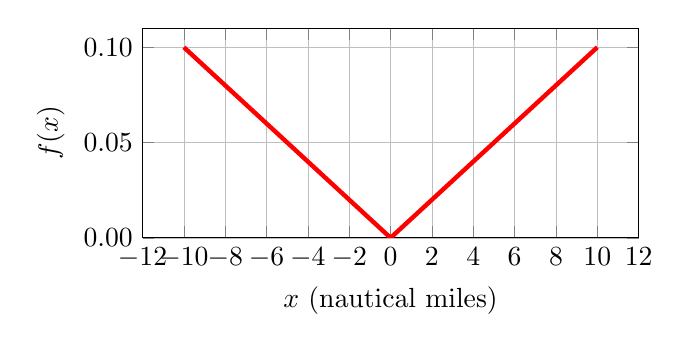
\begin{tikzpicture}
            \begin{axis}[
                width=0.65\textwidth,
                height=0.35\textwidth,
                xmin=-12, xmax=12,
                ymin=0, ymax=0.11,
                xtick={-12,-10,-8,-6,-4,-2,0,2,4,6,8,10,12},
                ytick={0.00,0.05,0.10},
                yticklabels={0.00,0.05,0.10},
                grid=both,
                xlabel={$x$ (nautical miles)},
                ylabel={$f(x)$},
                major grid style={line width=0.2pt,draw=gray!50},
                minor grid style={line width=0.1pt,draw=gray!20}
            ]
                \addplot[red, ultra thick] coordinates {(-10,0.10) (0,0) (10,0.10)};
            \end{axis}
        \end{tikzpicture}
        \captionof{figure}{Probability density function $f(x)$ governing the target's lateral position.}
        \label{fig:probability-density-function}
    \end{center}\medskip

    Under this specific spatial density, the probability that the target enters within the central region $[-5, 5]$ is given by the area under $f(x)$:
    \[
        P(-5 \le X \le 5) = \int_{-5}^{5} f(x)\dx = 0.25.
    \]
    Conversely, the probability that the target enters along the outer regions $[-10, -5] \cup [5, 10]$ is $0.75$.\medskip

    By integrating probabilistic geometric detection sweep coverage across time, the overall probability of detecting a target ($P_{\text{det}}$) can be derived analytically as:
    \[
        P_{\text{det}} = \left\{ \frac{4R^{3}}{3D^{3}} \left(1 + \left(\frac{V}{U}\right)^{2}\right) - \frac{2R^{2}}{D^{2}} \sqrt{1 + \left(\frac{V}{U}\right)^{2}} + \frac{2R}{D} \right\} \sqrt{1 + \left(\frac{V}{U}\right)^{2}}
    \]

    \paragraph{Example Calculation}
    Given parameters $D = 20\text{ nm}$, $R = 4\text{ nm}$, observer speed $V = 18\text{ knots}$, and target speed $U = 12\text{ knots}$:
    \[
        P_{\text{det}} \approx 0.5236 \quad (\text{\SI{52.36}{\percent}}).
    \]
\end{example}

\newpage

% ==============================================================================
% CHAPTER 2: PROBABILITY FOUNDATIONS
% ==============================================================================

\section*{Probability Concepts and Axioms}

We start by formalizing a concept that can be used to study random phenomena.

\begin{definition}[Probability model]
    A \emph{probability model} is characterized through the following three properties:\medskip

    \begin{itemize}\setlength\itemsep{1em}
        \item \textbf{Random Experiment}: a process or procedure that leads to one of several possible outcomes, where the precise outcome cannot be predicted with certainty in advance.
        \item \textbf{Sample Space ($S$)}: the set of all possible outcomes of a random experiment.
        \item \textbf{Event ($A, B, \dots$)}: any subset of outcomes contained within the sample space $S$.
    \end{itemize}
\end{definition}

\begin{example}[Target engagement]
    Consider an engagement model where a military weapon system engages a target iteratively until the target is successfully eliminated.\medskip

    \begin{itemize}\setlength\itemsep{1em}
        \item Let $h$ represent a hit (target destroyed) and $m$ represent a miss.
        \item The sample space is infinite and countable:
        \[S = \set{h, mh, mmh, mmmh, \ldots}\]
        \item Define Event $A$ as \enquote{eliminating the target in no more than 3 attempts}:
        \[A = \set{h, mh, mmh} \subset S\]
        \item Define Event $B$ as "requiring at least 2 attempts to eliminate the target":
        \[B = \set{mh, mmh, mmmh, \ldots} \subset S\]
    \end{itemize}
\end{example}

\paragraph{Set Operations on Events}
\begin{itemize}\setlength\itemsep{1em}
    \item \textbf{Complement ($A'$ or $A^c$)}: The event consisting of all outcomes in $S$ that are not in $A$ (not$\text{-}A$).
    \item \textbf{Intersection ($A \cap B$)}: The event containing outcomes that belong to \textit{both} $A$ and $B$.
    \item \textbf{Union ($A \cup B$)}: The event containing outcomes that belong to $A$, or $B$, or both.
    \item \textbf{Mutually exclusive (disjoint)}: Two events $A$ and $B$ are mutually exclusive if they share no common outcomes, meaning $A \cap B = \emptyset$.
\end{itemize}

Applying these set operations to our engagement model:
\begin{align*}
    B' &= \set{h} && \text{The target is eliminated on the very first attempt.} \\
    A \cap B &= \set{mh, mmh} && \text{The target is eliminated on exactly the 2nd or 3rd attempt.} \\
    A \cup B &= S && \text{Guaranteed outcome (the certain event).}
\end{align*}

\begin{definition}[Axioms of probability]
    Let $S$ be a sample space associated with a random experiment.
    A probability function $P$ is a real-valued function that assigns to each event $E \subset S$ a real number $P(E)$,
    satisfying the three formal Axioms of Probability:

    \begin{enumerate}\setlength\itemsep{1em}
        \item[\textbf{(A1)}] \textbf{Certain Event}: $P(S) = 1$ (the probability of the entire sample space is $1$).
        \item[\textbf{(A2)}] \textbf{Non-negativity}: $0 \le P(E) \le 1$ for any event $E \subset S$.
        \item[\textbf{(A3)}] \textbf{Mutual Exclusivity}: If $E_1$ and $E_2$ are pairwise mutually exclusive events ($E_1 \cap E_2 = \emptyset$), then:
        \[
            P(E_1 \cup E_2) = P(E_1) + P(E_2)
        \]
    \end{enumerate}
\end{definition}

\subsection*{Core Probability Rules}

From the foundational axioms, we derive the fundamental algebraic rules of probability theory:

\begin{itemize}\setlength\itemsep{1em}
    \item[\textbf{(R1)}] \textbf{Impossible Event}: $P(\emptyset) = 0$.
    \item[\textbf{(R2)}] \textbf{Complement Rule}: $P(A') = 1 - P(A)$.
    \item[\textbf{(R3.1)}] \textbf{General Addition Rule (Two Events)}: 
    \[
        P(A \cup B) = P(A) + P(B) - P(A \cap B)
    \]
\end{itemize}

\begin{center}
    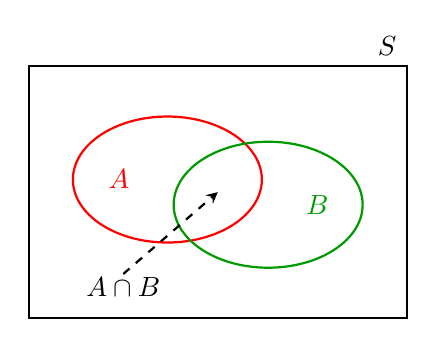
\begin{tikzpicture}[scale=0.8]
        \draw[thick] (0,0) rectangle (6,4) node[above left] {$S$};
        \draw[red, thick] (2.2,2.2) ellipse (1.5 and 1.0) node[left=10pt] {$A$};
        \draw[green!60!black, thick] (3.8,1.8) ellipse (1.5 and 1.0) node[right=10pt] {$B$};
        \node at (1.5,0.5) {$A \cap B$};
        \draw[-stealth, thick, dashed] (1.5,0.7) -- (3,2);
    \end{tikzpicture}
    \captionof{figure}{If you compute the probability $P(A \cup B)$, adding the probabilities $P(A)$ and $P(B)$ means you have counted the probability for the intersection $P(A \cap B)$ twice.}
    \label{fig:probability-rules}
\end{center}

\begin{proofbox}[(R3.1)]
    Using set decomposition, we express $A \cup B$ and $B$ as unions of disjoint sets:
    \[
        A \cup B = A \cup (B \cap A') \quad \text{and} \quad B = (A \cap B) \cup (B \cap A')
    \]
    Applying Axiom (A3) to both disjoint decompositions gives:
    \begin{align*}
        P(A \cup B) &= P(A) + P(B \cap A') \\
        P(B) &= P(A \cap B) + P(B \cap A') \implies P(B \cap A') = P(B) - P(A \cap B)
    \end{align*}
    Substituting $P(B \cap A')$ back into the first expression yields the General Addition Rule:
    \[
        P(A \cup B) = P(A) + P(B) - P(A \cap B)
    \]
\end{proofbox}
\begin{center}
    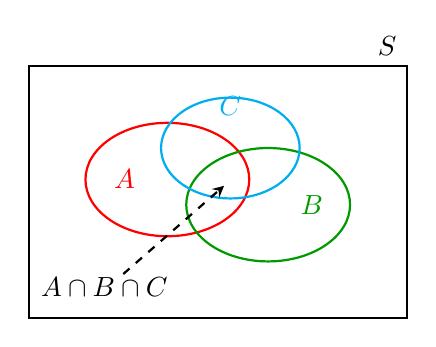
\begin{tikzpicture}[scale=0.8]
        \draw[thick] (0,0) rectangle (6,4) node[above left] {$S$};
        \draw[red, thick] (2.2,2.2) ellipse (1.3 and 0.9) node[left=8pt] {$A$};
        \draw[green!60!black, thick] (3.8,1.8) ellipse (1.3 and 0.9) node[right=8pt] {$B$};
        \draw[cyan, thick] (3.2,2.7) ellipse (1.1 and 0.8) node[above=8pt] {$C$};
        \node at (1.2,0.5) {$A \cap B \cap C$};
        \draw[-stealth, thick, dashed] (1.5,0.7) -- (3.1,2.1);
    \end{tikzpicture}
    \captionof{figure}{Venn diagram for the union of three overlapping events $A$, $B$, and $C$.}
    \label{fig:2.2}
\end{center}

\begin{itemize}
    \item[\textbf{(R3.2)}] \textbf{Addition Rule for Three Events}:
    \[
        P(A \cup B \cup C) = P(A) + P(B) + P(C) - P(A \cap B) - P(A \cap C) - P(B \cap C) + P(A \cap B \cap C)
    \]
\end{itemize}

\begin{exercise}[tossing two dice]
    Consider rolling two fair six-sided dice. The sample space $S$ consists of $36$ equally likely ordered pairs $(i, j)$ for $i, j \in \{1, \dots, 6\}$.
    \begin{itemize}\setlength\itemsep{1em}
        \item Let $A$ = \enquote{sum is at least 10} $= \set{(4,6), (5,5), (5,6), (6,4), (6,5), (6,6)}$.
        \item Let $B$ = \enquote{sum is no more than 10}.
    \end{itemize}

    Calculating the corresponding probabilities $P(A)$, $P(B)$, $P(A \cap B)$ and $P(A \cup B)$.
\end{exercise}

\begin{solution}
    \begin{align*}
        P(A) &= \frac{|A|}{36} = \frac{6}{36} = \frac{1}{6} \\
        P(B) &= 1 - P(B') = 1 - P(\text{sum is 11 or 12}) = 1 - \frac{3}{36} = \frac{33}{36} = \frac{11}{12} \\
        P(A \cap B) &= P(\text{sum is exactly 10}) = P(\{(4,6), (5,5), (6,4)\}) = \frac{3}{36} = \frac{1}{12} \\
        P(A \cup B) &= P(A) + P(B) - P(A \cap B) = \frac{6}{36} + \frac{33}{36} - \frac{3}{36} = \frac{36}{36} = 1
    \end{align*}
\end{solution}

\subsection*{Conditional Probability}

Conditional probability measures the probability of an event $B$ occurring given that another event $A$ has already occurred.

\begin{center}
    \begin{tikzpicture}[scale=0.8]
        \draw[thick] (0,0) rectangle (6,4) node[above left] {$S$};
        \fill[pattern=dots, pattern color=red!60] (2.2,2.2) ellipse (1.5 and 1.0);
        \draw[red, ultra thick] (2.2,2.2) ellipse (1.5 and 1.0) node[left=10pt] {$A$};
        \draw[green!60!black, thick] (3.8,1.8) ellipse (1.5 and 1.0) node[right=10pt] {$B$};
        \node at (1.5,0.5) {$A \cap B$};
        \draw[->, thick, dashed] (1.5,0.7) -- (3,2);
    \end{tikzpicture}
    \captionof{figure}{Reduced sample space when conditioning on the occurrence of event $A$.}
    \label{fig:independence}
\end{center}

\begin{definition}[conditional probability]
Formally, for any event $A$ such that $P(A) > 0$, the \emph{conditional probability} of $B$ given $A$ is defined as:
\[
    P(B|A) = \frac{P(A \cap B)}{P(A)}
\]
\end{definition}

\subsection*{Multiplication and Total Probability Rules}

Rearranging the definition of conditional probability provides the \textbf{Multiplication Rules}:
\begin{itemize}\setlength\itemsep{1em}
    \item[\textbf{(R4.1)}] $P(A \cap B) = P(A) \cdot P(B|A)$
    \item[\textbf{(R4.2)}] $P(A \cap B) = P(B) \cdot P(A|B)$
\end{itemize}

\paragraph{Total Probability Rule (Two-Event Form)}
For any event $B$ and condition event $A$:
\begin{itemize}
    \item[\textbf{(R5)}] $P(B) = P(B|A)P(A) + P(B|A')P(A')$
\end{itemize}

\begin{proofbox}[(R5)]
    Decomposing $B$ into mutually exclusive components relative to $A$:
    \[
        B = (B \cap A) \cup (B \cap A')
    \]
    Taking probabilities using Axiom (A.3) and applying Rule (R4.2) gives:
    \[
        P(B) = P(B \cap A) + P(B \cap A') = P(B|A)P(A) + P(B|A')P(A')
    \]
\end{proofbox}

\begin{example}[semiconductor quality control]
    Suppose that in semiconductor manufacturing, the probability is $0.10$ that a chip subjected to high levels of contamination during manufacturing causes a product failure.
    The probability is $0.005$ that a chip not subjected to high contamination levels during manufacturing causes a product failure.
    In a particular production run, \SI{20}{\percent} of the chips are subject to high levels of contamination.
    What is the probability that a product using one of these chips fails?
\end{example}

\begin{solution}
    It helps to look at this problem by defining relevant events that we can apply the probability rules to, given the information:

    Let $A$ be the event \enquote{chip is subjected to high levels of contamination}, and $B$ the event \enquote{semiconductor fails}.
    We know the following probabilities already:\medskip

    \begin{itemize}\setlength\itemsep{1em}
        \item Probability of failure given high contamination: $P(B|A) = 0.10$.
        \item Probability of failure given normal conditions: $P(B|A') = 0.005$.
        \item Proportion of chips subjected to high contamination: $P(A) = 0.20$ (thus $P(A') = 0.80$).
    \end{itemize}
    We determine the total probability of chip failure $P(B)$ using a probability tree diagram:\medskip

    \begin{center}
        \begin{tikzpicture}
            \node (start) at (0,0) {};

            \node[red] (child1) at (2,2) {$A$};
            \node[red] (child2) at (2,-2) {$A'$};

            \node[green!50!black] (child11) at (4,3) {$B$};
            \node[green!50!black] (child12) at (4,1) {$B'$};
            \node[green!50!black] (child21) at (4,-1) {$B$};
            \node[green!50!black] (child22) at (4,-3) {$B'$};

            \draw[arrow] (start) -- node[midway,sloped,above] {$0.2$} (child1);
            \draw[arrow] (start) -- node[midway,sloped,below] {$0.8$} (child2);
            \draw[arrow] (child1) -- node[midway,sloped,above] {$0.1$} (child11);
            \draw[arrow] (child1) -- node[midway,sloped,below] {$0.9$} (child12);
            \draw[arrow] (child2) -- node[midway,sloped,above] {$0.005$} (child21);
            \draw[arrow] (child2) -- node[midway,sloped,below] {$0.995$} (child22);

            \node[right of=child11, xshift=5cm] (prob-child11) {$0.2 \cdot 0.1 = 0.02$\qquad \qquad {\color{blue} $P(B|A)\cdot P(A)$}};
            \node[right of=child21, xshift=5cm] (prob-child21) {$0.8 \cdot 0.005 = 0.004$\qquad \qquad {\color{blue} $P(B|A')\cdot P(A')$}};

        \end{tikzpicture}
        \captionof{figure}{Probability tree structure for semiconductor contamination and failure analysis.}
        \label{fig:probability-tree}
    \end{center}\medskip

    Summing the path probabilities yields:
    \[
        P(B) = P(B|A)\cdot P(A) + P(B|A')\cdot P(A') = 0.020 + 0.004 = \mathbf{0.024} \quad (\text{\SI{2.4}{\percent}})
    \]
\end{solution}

\paragraph{General Law of Total Probability}
If the sample space $S$ is partitioned into $k$ mutually exclusive and exhaustive events $A_1, A_2, \dots, A_k$ (such that $\bigcup_{i=1}^{k} A_i = S$ and $A_i \cap A_j = \emptyset$ for $i \neq j$), then for any event $B$:
\[
    P(B) = \sum_{i=1}^{k} P(B|A_i) \cdot P(A_i)
\]